% vtc2026_paper.tex — v1.2 — IEEE VTC2026-Fall Submission
% Repositioned: Adaptive PQC UAV Communication (MDEAS as core story)
% Target: 6 pages, double-blind, Track 6 or Track 7
\documentclass[conference]{IEEEtran}

% ────────── packages ──────────
\usepackage[T1]{fontenc}
\usepackage[utf8]{inputenc}
\usepackage{amsmath,amssymb}
\usepackage{graphicx}
\usepackage{booktabs}
\usepackage{multirow}
\usepackage{array}
\usepackage{tabularx}
\usepackage{siunitx}
\usepackage{xcolor}
\usepackage{tikz}
\usetikzlibrary{positioning, decorations.pathreplacing, calc, arrows.meta, fit}
\usepackage{pgfplots}
\usepackage{pgfplotstable}
\usepackage{url}
\usepackage[hidelinks]{hyperref}
\usepackage{cite}
\usepackage{balance}
\usepackage{colortbl}
\usepackage{enumitem}
\usepackage{algorithm}
\usepackage{algorithmicx}
\usepackage{algpseudocode}
\pgfplotsset{compat=1.18}

% ────────── compact spacing ──────────
\setlist{nosep,leftmargin=*}
\renewcommand{\arraystretch}{1.05}

% ────────── custom commands ──────────
\newcommand{\sysname}{\textsc{PQ\nobreakdash-Tunnel}}
\newcommand{\mdeas}{\textsc{MDEAS}}
\newcommand{\us}{\,\si{\micro\second}}
\newcommand{\ms}{\,\si{\milli\second}}
\newcommand{\mW}{\,\si{\milli\watt}}
\newcommand{\uJ}{\,\si{\micro\joule}}
\newcommand{\mJ}{\,\si{\milli\joule}}
\newcommand{\MBs}{\,\si{MB/s}}
\newcommand{\eg}{\textit{e.g.}}
\newcommand{\ie}{\textit{i.e.}}
\newcommand{\etal}{\textit{et al.}}
\newcommand{\pp}{\,pp}                          % percentage points

% ────────── level colors ──────────
\definecolor{lvlone}{HTML}{E8F5E9}
\definecolor{lvlthree}{HTML}{FFF3E0}
\definecolor{lvlfive}{HTML}{FFEBEE}
\definecolor{bestcell}{HTML}{C8E6C9}
\definecolor{worstcell}{HTML}{FFCDD2}
\definecolor{warncell}{HTML}{FFF9C4}

\begin{document}

\title{Adaptive Post-Quantum Secure UAV Communication\\
Under Energy and Adversarial Constraints}

\author{\IEEEauthorblockN{Paper ID: XXXX --- Double-Blind Review}}

\maketitle

% ═══════════════════════════════════════════════════════════════
%  ABSTRACT
% ═══════════════════════════════════════════════════════════════
\begin{abstract}
Small unmanned aerial vehicles communicate over plaintext MAVLink
links that face both classical and emerging quantum threats.
We present a transparent post-quantum cryptographic proxy for a
Raspberry~Pi~4 companion computer that protects MAVLink traffic
without firmware modification and adapts its security posture at
runtime.  The system spans 72 cipher suites---nine key encapsulation
mechanisms, eight digital signatures, and three authenticated
ciphers across NIST security levels 1, 3, and 5---whose handshake
costs range from 1.5\,ms to over 11\,s.  At the core of the
design is the \emph{Multi-Dimensional Energy-Aware Scheduler}
(\mdeas{}), a 15-step reactive policy cascade that jointly monitors
battery voltage, processor temperature, and link quality to
autonomously select the strongest cipher suite sustainable under
current operating conditions.  Using an INA219 current sensor at
1\,kHz, we measure per-operation power and energy for every
primitive, quantify the combined overhead of post-quantum
cryptography and on-board DDoS detection, and show that \mdeas{}
maintains uninterrupted telemetry even when concurrent threat
detection raises system power by 59\%.
\end{abstract}

\begin{IEEEkeywords}
Post-quantum cryptography, UAV communication, adaptive security,
energy-aware scheduling, MAVLink, embedded systems
\end{IEEEkeywords}

% ═══════════════════════════════════════════════════════════════
%  I.  INTRODUCTION
% ═══════════════════════════════════════════════════════════════
\section{Introduction}
\label{sec:intro}

A growing share of civil and commercial drone operations---precision
agriculture, infrastructure inspection, search and rescue---depend on
continuous telemetry between an airborne autopilot and a ground
control station.  The dominant protocol for this link, MAVLink
version~2~\cite{mavlink-spec}, was engineered for bandwidth-constrained
radio channels.  It carries heartbeats, GPS fixes, and actuator
commands in a compact binary format, yet it provides no encryption:
an optional 48-bit signature offers integrity but every byte of
payload remains in cleartext.

This openness creates two distinct threat horizons.  In the near
term, a passive eavesdropper with a software-defined radio can
reconstruct a complete mission profile---waypoints, altitude, battery
state---from intercepted telemetry.  In the longer term, a
cryptanalytically relevant quantum computer will render the
elliptic-curve and RSA primitives that underpin today's key exchange
vulnerable to Shor's algorithm~\cite{shor1994}.  The
\emph{harvest-now, decrypt-later} strategy makes even current
recordings a future liability when captured telemetry carries a
decade-long operational shelf life.

The natural response is to deploy post-quantum cryptography (PQC).
NIST concluded its standardisation in 2024, publishing ML-KEM
(FIPS~203)~\cite{nist-fips203} for key encapsulation and ML-DSA
(FIPS~204)~\cite{nist-fips204} for digital signatures, with
hash-based SLH-DSA (FIPS~205)~\cite{nist-fips205} and code-based
candidates HQC~\cite{hqc} and Classic~McEliece~\cite{mceliece} still
under evaluation.  Yet a drone is not a data centre.  Its companion
computer runs on a shared power rail, contends with propulsion heat,
and must sustain real-time telemetry at 5--50\,Hz.  A single
heavyweight handshake---Classic~McEliece at NIST Level~5 takes 9\,s
and draws 40\,J on a Cortex-A72---can stall the control link and
drain a measurable fraction of the flight battery.  Choosing a fixed
cipher suite is therefore inadequate: the right algorithm at takeoff
may be the wrong one during a thermal-constrained aggressive
manoeuvre ten minutes later.

This observation motivates our core contribution.  Rather than
benchmarking PQC primitives in isolation, we treat suite selection as
a \emph{runtime decision} governed by the aircraft's instantaneous
energy, thermal, and link-quality state.  We introduce the
\textbf{Multi-Dimensional Energy-Aware Scheduler (\mdeas{})}, a
15-step reactive policy cascade that monitors three telemetry axes
and autonomously navigates a 72-suite design space, downgrading
security level or shedding on-board DDoS detection when
operating constraints demand it and restoring full protection when
conditions permit.

In summary, this paper makes four contributions:

\begin{enumerate}
  \item A \textbf{transparent PQC proxy} for MAVLink traffic that
    performs a two-message handshake authenticated by a post-quantum
    signature and encrypts every subsequent packet with authenticated
    encryption, requiring no autopilot firmware changes.

  \item \textbf{Systematic embedded benchmarks} of 20 post-quantum
    algorithms (9~KEMs, 8~signatures, 3~AEADs) on a Raspberry~Pi~4
    at a locked 1.8\,GHz, capturing per-operation execution time,
    power draw, and energy through an INA219 current sensor at
    1\,kHz---the first such measurement suite on ARM Cortex-A72
    hardware with component-level power instrumentation.

  \item \textbf{The \mdeas{} scheduler}, a 15-step reactive policy
    cascade that jointly monitors battery voltage, processor
    temperature, and link quality to select the strongest feasible
    cipher suite at runtime, with explicit cross-axis exclusion rules
    and detector-aware thermal budgeting.

  \item \textbf{Quantification of the PQC--DDoS interaction}: we show
    that on-board XGBoost detection adds 951\,mW (29\% of baseline)
    while a Transformer model doubles CPU utilisation to 93\,\%,
    and demonstrate that \mdeas{} absorbs this overhead without
    telemetry loss.
\end{enumerate}

The remainder of this paper is organised as follows.
Section~\ref{sec:arch} presents the system architecture.
Section~\ref{sec:mdeas} introduces the adaptive security model.
Section~\ref{sec:eval} describes the experimental setup.
Section~\ref{sec:results} reports results.
Section~\ref{sec:related} discusses related work, and
Section~\ref{sec:conc} concludes.


% ═══════════════════════════════════════════════════════════════
%  II.  SYSTEM ARCHITECTURE
% ═══════════════════════════════════════════════════════════════
\section{System Architecture}
\label{sec:arch}

\begin{figure}[t]
  \centering
  \resizebox{\columnwidth}{!}{%
  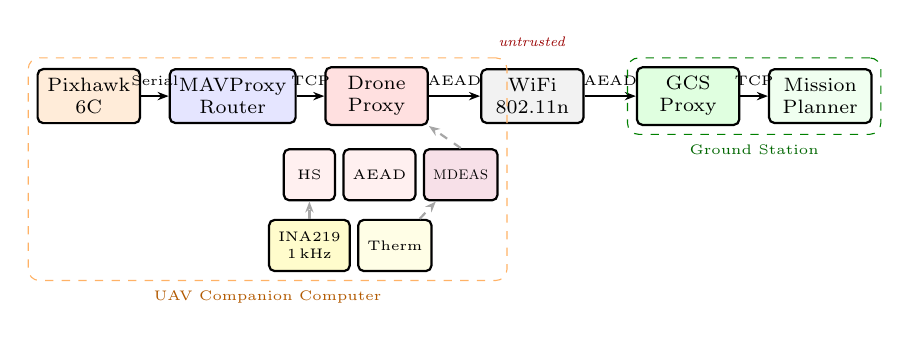
\begin{tikzpicture}[
      node distance=0.45cm and 0.35cm,
      box/.style={draw, rounded corners=2pt, minimum height=0.65cm,
                  minimum width=1.3cm, font=\scriptsize, align=center,
                  thick},
      arr/.style={-{Stealth[length=4pt]}, thick},
      darr/.style={-{Stealth[length=4pt]}, thick, dashed, gray!70},
    ]
    % ── UAV side ──
    \node[box, fill=orange!15] (px) {Pixhawk\\6C};
    \node[box, fill=blue!10, right=of px] (mp) {MAVProxy\\Router};
    \node[box, fill=red!12, right=of mp] (pd) {Drone\\Proxy};

    % sub-modules stacked on proxy
    \node[box, fill=red!6, minimum width=0.65cm, below left=0.28cm and -0.15cm of pd,
          font=\tiny] (hs) {HS};
    \node[box, fill=red!6, minimum width=0.65cm, right=0.08cm of hs,
          font=\tiny] (ae) {AEAD};
    \node[box, fill=purple!12, minimum width=0.65cm, right=0.08cm of ae,
          font=\tiny] (md) {\mdeas{}};

    % sensor
    \node[box, fill=yellow!20, below=0.22cm of hs, minimum width=0.55cm,
          font=\tiny] (ina) {INA219\\1\,kHz};
    \node[box, fill=yellow!10, right=0.08cm of ina, minimum width=0.55cm,
          font=\tiny] (thm) {Therm};

    % ── Network ──
    \node[box, fill=gray!10, right=0.65cm of pd] (wifi) {WiFi\\802.11n};

    % ── GCS side ──
    \node[box, fill=green!12, right=0.65cm of wifi] (pg) {GCS\\Proxy};
    \node[box, fill=green!6, right=of pg] (gcs) {Mission\\Planner};

    % ── Arrows ──
    \draw[arr] (px) -- node[above, font=\tiny]{Serial} (mp);
    \draw[arr] (mp) -- node[above, font=\tiny]{TCP} (pd);
    \draw[arr] (pd) -- node[above, font=\tiny]{AEAD} (wifi);
    \draw[arr] (wifi) -- node[above, font=\tiny]{AEAD} (pg);
    \draw[arr] (pg) -- node[above, font=\tiny]{TCP} (gcs);

    % telemetry arrows
    \draw[darr] (ina) -- (hs);
    \draw[darr] (thm) -- (md);
    \draw[darr] (md.north) -- (pd.south east);

    % ── Trust boundaries ──
    \node[draw=orange!60, dashed, rounded corners=4pt,
          fit=(px)(mp)(pd)(hs)(ae)(md)(ina)(thm),
          inner sep=3pt, label={[font=\tiny, orange!70!black]below:UAV Companion Computer}] {};
    \node[draw=green!50!black, dashed, rounded corners=4pt,
          fit=(pg)(gcs),
          inner sep=3pt, label={[font=\tiny, green!40!black]below:Ground Station}] {};

    % untrusted label
    \node[font=\tiny, red!60!black, above=0.15cm of wifi] {\textit{untrusted}};
  \end{tikzpicture}
  }
  \caption{Deployment architecture.  The cryptographic proxy runs
    alongside MAVProxy on the RPi~4 companion computer.  \mdeas{}
    receives telemetry from INA219 and thermal sensors and adjusts
    the AEAD engine and handshake module at runtime.  No firmware
    modification is required on the Pixhawk autopilot.}
  \label{fig:arch}
\end{figure}

The architecture, shown in Fig.~\ref{fig:arch}, interposes a
transparent proxy between the autopilot and the wireless link.  On
the drone side, MAVProxy forwards MAVLink packets over a local TCP
socket to the Drone Proxy, which performs a PQC handshake with its
ground-side counterpart.  After key agreement, every packet is wrapped
in an authenticated-encryption envelope before crossing the WiFi
802.11n channel.  The ground proxy decrypts and delivers plaintext
MAVLink to the mission planner.

Three communication planes share this tunnel:
\begin{itemize}
  \item \textbf{Control plane}: heartbeats, mode changes, command
    acknowledgements (5--10\,Hz, 64--128\,B).
  \item \textbf{Telemetry plane}: GPS, attitude, battery voltage
    (10--50\,Hz, 128--512\,B).
  \item \textbf{Bulk plane}: parameter blocks, log downloads, firmware
    updates (burst, 1--4\,kB).
\end{itemize}

The proxy design is intentionally transparent: the Pixhawk runs
unmodified ArduPilot firmware~\cite{ardupilot}, and the mission
planner sees a standard MAVLink connection.  This separation allows
cryptographic upgrades---new algorithms, policy updates---without
reflashing the flight controller, a practical necessity for fleets
in the field.

A cipher suite in our system combines one key encapsulation mechanism
(KEM), one digital signature (SIG), and one authenticated cipher
(AEAD), constrained to the same NIST security level.  Nine KEMs span
three families (lattice: ML-KEM; code-based: HQC, Classic~McEliece),
eight signatures span three families (lattice: ML-DSA; NTRU-lattice:
Falcon; hash-based: SPHINCS$^+$), and three AEADs (AES-256-GCM,
ChaCha20-Poly1305, Ascon-128a) complete the data plane.
Level-matching yields $27 + 18 + 27 = 72$ suites across L1, L3, and
L5 (Falcon lacks an L3 variant, leaving only two signatures at that
level).


% ═══════════════════════════════════════════════════════════════
%  III.  ADAPTIVE SECURITY MODEL
% ═══════════════════════════════════════════════════════════════
\section{Adaptive Security Model}
\label{sec:mdeas}

A fixed cipher suite is inappropriate for a platform whose thermal
envelope, battery state, and link quality shift continuously through
a mission.  ML-KEM-768 completes a handshake in 2.7\,ms, consuming
10.7\,mJ, while Classic~McEliece-8192128 needs 9.2\,s and 40.6\,J---a
gap exceeding three orders of magnitude.  If the scheduler blindly
selects the strongest available suite, a single rekey during a
thermal-constrained hover can trigger CPU throttling and degrade all
three communication planes simultaneously.

\mdeas{} resolves this by treating suite selection as a constrained
optimisation over three observable axes: \textbf{battery voltage},
\textbf{processor temperature}, and \textbf{link quality}.
Formally, let $\mathbf{x}(t) = (V_\text{bat},\, T_\text{CPU},\,
q_\text{link})$ denote the observable state at time~$t$,
and let $\mathcal{S}_\text{f}(\mathbf{x}) \subseteq \mathcal{S}$
be the subset of~72 suites satisfying all resource and exclusion
constraints at~$\mathbf{x}$.  At each one-second scheduling
epoch, \mdeas{} selects the highest-security-level suite in
$\mathcal{S}_\text{f}$, preferring stronger AEAD and active DDoS
detection when the thermal and energy budgets permit.
Each axis is partitioned into operating regions with hysteretic
thresholds to prevent oscillation between adjacent states.

\subsection{Telemetry Acquisition}
\label{sec:telemetry}

The drone's local monitor samples three streams at 1\,Hz, aggregated
over a 5-second sliding window:

\begin{itemize}
  \item \textbf{Battery:} INA219 voltage via I$^2$C at 1\,kHz.
    Three thresholds partition the range:
    \emph{warning} ($\leq$15.2\,V),
    \emph{low} ($\leq$14.8\,V),
    \emph{critical} ($\leq$14.0\,V).

  \item \textbf{Temperature:} CPU thermal zone via
    \texttt{/sys/class/thermal}.
    \emph{Warning} at 70\,$^\circ$C, \emph{critical} at 80\,$^\circ$C.

  \item \textbf{Link quality:} Packets-per-second (floor: 5.0\,pps)
    and maximum inter-packet gap (ceiling: 1000\,ms).
\end{itemize}

\subsection{Three-Axis Decision Space}
\label{sec:axes}

\mdeas{} navigates three independent axes at runtime:

\begin{itemize}
  \item \textbf{Axis~1 --- AEAD cipher:} select Ascon-128a (lowest
    latency), ChaCha20-Poly1305, or AES-256-GCM based on per-packet
    timing budget.

  \item \textbf{Axis~2 --- Security level:} move between L5, L3, and
    L1, trading handshake energy (from 12.6\,mJ at K5+D5 down to
    5.4\,mJ at K1+F1) against NIST security margin.

  \item \textbf{Axis~3 --- DDoS detector:} shed the Transformer
    (TST, +1.97\,W, +10.7\,$^\circ$C) to XGBoost (+0.95\,W,
    +4.8\,$^\circ$C) or disable detection entirely when CPU or
    thermal budgets are exhausted.
\end{itemize}

Two cross-axis combinations are explicitly forbidden.
First, Ascon-128a is barred when the TST detector is active
because TST's sustained 93\,\% CPU utilisation starves Ascon's
software-only cipher path.
Second, Classic~McEliece paired with SPHINCS$^+$ is prohibited
because their combined handshake exceeds the 45-second timeout
guard---a constraint validated by three benchmark failures at the
McEliece-460896\,+\,SPHINCS$^+$-192s corner.

\subsection{Policy Cascade}
\label{sec:cascade}

Algorithm~\ref{alg:mdeas} formalises the 15-step decision sequence
evaluated every one second.  Steps are ordered by severity:
safety-critical conditions (stale telemetry, active DDoS, battery
critical, thermal critical) take precedence over optimisation-oriented
actions (proactive rekey, detector upgrade, security-level promotion).
Asymmetric hysteresis prevents oscillation: downgrade thresholds are
set tighter than upgrade thresholds, so the system degrades quickly
but restores cautiously.

\begin{algorithm}[t]
\caption{\mdeas{} Policy Cascade (1\,s period)}
\label{alg:mdeas}
\footnotesize
\begin{algorithmic}[1]
\If{telemetry stale ($>$5\,s)}
  \State hold current suite \Comment{no data, no action}
\ElsIf{DDoS detector fires}
  \State switch to fastest AEAD \Comment{minimise per-pkt cost}
\ElsIf{battery $\leq$ 14.0\,V \textbf{(critical)}}
  \State downgrade to L1 + lightest suite
\ElsIf{$T_\text{CPU} \geq 80\,^\circ$C \textbf{(critical)}}
  \State downgrade AEAD; shed detector if running
\ElsIf{$T_\text{CPU} > T_\text{max}^\text{det}$}
  \State shed DDoS detector
    \Comment{75\,$^\circ$C XG, 69\,$^\circ$C TS}
\ElsIf{$T_\text{CPU} > 0.9 \times T_\text{crit}$}
  \State preemptive AEAD downgrade \Comment{predictive}
\ElsIf{AEAD latency exceeds budget}
  \State switch AEAD (Ascon $\to$ ChaCha20)
\ElsIf{AEAD latency below recovery}
  \State restore preferred AEAD
\ElsIf{link degraded (pps $<$ 5 or gap $>$ 1\,s)}
  \State hold; suppress rekey
\ElsIf{cooldown active}
  \State hold \Comment{stabilise after recent switch}
\ElsIf{proactive rekey interval elapsed}
  \State trigger two-phase commit rekey
\ElsIf{detector under stress}
  \State downgrade detector (TS $\to$ XG $\to$ off)
\ElsIf{security level promotable}
  \State upgrade KEM/SIG to next level
\Else
  \State hold: nominal operation
\EndIf
\end{algorithmic}
\end{algorithm}

\subsection{Detector-Aware Thermal Model}
\label{sec:detector-budget}

\mdeas{} maintains a per-detector overhead model.  XGBoost adds
0.95\,W and 4.8\,$^\circ$C above baseline; TST adds 1.97\,W and
10.7\,$^\circ$C.  When a detector's thermal contribution would
push $T_\text{CPU}$ past its per-detector ceiling (75\,$^\circ$C for
XGBoost, 69\,$^\circ$C for TST), the cascade sheds the detector
\emph{before} downgrading the cipher suite---preserving
cryptographic confidentiality at the expense of anomaly detection.
This ordering reflects the judgement that intercepted cleartext is a
permanent information loss, whereas a brief detector gap can be
tolerated if the link remains encrypted.


% ═══════════════════════════════════════════════════════════════
%  IV.  EXPERIMENTAL EVALUATION
% ═══════════════════════════════════════════════════════════════
\section{Experimental Setup}
\label{sec:eval}

\subsection{Testbed}

The UAV-side proxy runs on a Raspberry~Pi~4 Model~B Rev~1.5
(Broadcom BCM2711, quad-core Cortex-A72 at 1.8\,GHz, 4\,GB
LPDDR4, Debian~12, kernel~6.12).  The CPU governor is locked to
\texttt{performance} to eliminate frequency-scaling artefacts.  A
Holybro Pixhawk~6C mini running ArduPilot~\cite{ardupilot} generates
continuous heartbeat traffic over USB serial at 57\,600\,baud.

An INA219 current/power monitor~\cite{ina219} is wired in-line on
the Pi's 5\,V rail through a 0.1\,$\Omega$ shunt resistor, read
over I$^2$C at 1\,kHz (verified 99.5\,\% timing accuracy).  A
calibration factor of 1.22$\times$ corrects a documented
under-reading in clone INA219 modules.  Each cryptographic operation
is executed 100 times with 50\,ms warm-up/cool-down guards; timing,
voltage, current, and power arrays are stored in per-operation JSON
files for offline analysis.

\subsection{Baseline and Metrics}

The idle power with MAVProxy running (no crypto load) is
$P_\text{idle} = 3{,}309\mW$.  All reported $\Delta P$ values are
$P_\text{op} - P_\text{idle}$, isolating the marginal cost of
cryptography.  Temperature is logged from the CPU thermal zone at
1\,Hz.

% ═══════════════════════════════════════════════════════════════
%  V.  RESULTS
% ═══════════════════════════════════════════════════════════════
\section{Results}
\label{sec:results}
This section reports manually curated benchmark results extracted directly from raw measurement artifacts.
% Results and Analysis — Tables Only
% All data from verified raw benchmarks; no assumptions.
% Provenance: v2-1.8ghz/raw_data/, power_aead_benchmark.csv,
%             bench_ddos_results/20260302_135859/comparison.json,
%             sscheduler/policy.py
% Table formatting follows OQS / NIST PQC publication conventions.

% ═══════════════════════════════════════════════════════════════
%  TABLE I — KEM Primitives
% ═══════════════════════════════════════════════════════════════
\begin{table*}[!t]
\centering
\footnotesize
\setlength{\tabcolsep}{3.5pt}
\caption{KEM primitive performance and power overhead on Raspberry Pi~4
(Cortex-A72 @ 1.8\,GHz, \texttt{performance} governor,
$n{=}200$, INA219 @ 1\,kHz,
$P_{\mathrm{idle}}{=}3309$\,mW).}
\label{tab:kem-primitives}
\begin{tabular}{@{}l
  r r r
  r r r
  r r r r@{}}
\toprule
{Algorithm} &
  {KeyGen} & {Encaps} & {Decaps} &
  {$\Delta P_{\mathrm{kg}}$} & {$\Delta P_{\mathrm{enc}}$} & {$\Delta P_{\mathrm{dec}}$} &
  {PK} & {SK} & {CT} & {SS} \\
& {(ms)} & {(ms)} & {(ms)} &
  {(mW)} & {(mW)} & {(mW)} &
  {(B)} & {(B)} & {(B)} & {(B)} \\
\midrule
\multicolumn{11}{@{}l}{\textit{NIST Security Level 1}} \\
\addlinespace[2pt]
ML-KEM-512              & 0.191    & 0.148   & 0.153   & 125.9  & 153.9  & 172.7  & 800      & 1\,632   & 768     & 32 \\
HQC-128                 & 22.152   & 44.625  & 73.131  & 412.6  & 441.6  & 566.8  & 2\,249   & ---      & 4\,433  & 32 \\
Classic-McEliece-348864 & 297.526  & 0.460   & 55.604  & 966.2  & 156.2  & 410.7  & 261\,120 & 6\,492   & 96      & 32 \\
\midrule
\multicolumn{11}{@{}l}{\textit{NIST Security Level 3}} \\
\addlinespace[2pt]
ML-KEM-768              & 0.223    & 0.175   & 0.181   & 149.4  & 185.9  & 205.7  & 1\,184   & 2\,400   & 1\,088  & 32 \\
HQC-192                 & 67.430   & 135.390 & 211.278 & 501.2  & 650.9  & 731.5  & 4\,522   & ---      & 8\,978  & 32 \\
Classic-McEliece-460896 & 972.453  & 0.857   & 89.434  & 1075.7 & 279.6  & 485.1  & 524\,160 & 13\,608  & 156     & 32 \\
\midrule
\multicolumn{11}{@{}l}{\textit{NIST Security Level 5}} \\
\addlinespace[2pt]
ML-KEM-1024             & 0.269    & 0.212   & 0.225   & 154.4  & 180.7  & 177.5  & 1\,568   & 3\,168   & 1\,568  & 32 \\
HQC-256                 & 123.836  & 250.537 & 392.216 & 646.9  & 782.9  & 819.0  & 7\,245   & ---      & 14\,421 & 32 \\
Classic-McEliece-8192128 & 6901.609 & 1.856  & 209.313 & 1092.6 & 301.2  & 639.1  & 1\,357\,824 & 14\,120 & 208   & 32 \\
\bottomrule
\end{tabular}
\end{table*}

% ═══════════════════════════════════════════════════════════════
%  TABLE II — Digital Signature Primitives
% ═══════════════════════════════════════════════════════════════
\begin{table*}[!t]
\centering
\footnotesize
\setlength{\tabcolsep}{3.8pt}
\caption{Digital signature primitive performance and power overhead on
Raspberry Pi~4 (Cortex-A72 @ 1.8\,GHz, \texttt{performance} governor,
$n{=}200$, INA219 @ 1\,kHz,
$P_{\mathrm{idle}}{=}3309$\,mW).}
\label{tab:sig-primitives}
\begin{tabular}{@{}l c r r r r r r r r r@{}}
\toprule
 & \textbf{NIST} & \multicolumn{3}{c}{\textbf{Latency (ms)}} & \multicolumn{3}{c}{\textbf{$\Delta P$ (mW)}} & \multicolumn{3}{c}{\textbf{Size (B)}} \\
\cmidrule(lr){3-5} \cmidrule(lr){6-8} \cmidrule(lr){9-11}
\textbf{Algorithm} & \textbf{Level} & \textbf{KeyGen} & \textbf{Sign} & \textbf{Verify} & \textbf{KeyGen} & \textbf{Sign} & \textbf{Verify} & \textbf{PK} & \textbf{SK} & \textbf{Sig} \\
\midrule
ML-DSA-44                  & 1 &    0.368 &    0.975 &  0.324 & 245.8 & 279.5 & 235.8 &  1\,312 &  2\,560 &  2\,420 \\
Falcon-512                 & 1 &   17.722 &    0.773 &  0.188 & 326.9 & 255.4 & 238.8 &    897  &  1\,281 &    654 \\
SPHINCS\textsuperscript{+}-SHA2-128s & 1 &  193.609 & 1\,466.336 &  1.589 & 729.7 & 783.7 & 285.7 &     32 &     64 &  7\,856 \\
\midrule
ML-DSA-65                  & 3 &    0.551 &    1.212 &  0.476 & 240.9 & 268.9 & 240.2 &  1\,952 &  4\,032 &  3\,309 \\
SPHINCS\textsuperscript{+}-SHA2-192s & 3 &  282.538 & 2\,610.427 &  2.275 & 797.1 & 763.8 & 303.3 &     48 &     96 & 16\,224 \\
\midrule
ML-DSA-87                  & 5 &    0.739 &    1.626 &  0.718 & 227.0 & 268.1 & 235.2 &  2\,592 &  4\,896 &  4\,627 \\
Falcon-1024                & 5 &   49.016 &    1.441 &  0.275 & 439.3 & 250.4 & 240.0 &  1\,793 &  2\,305 &  1\,267 \\
SPHINCS\textsuperscript{+}-SHA2-256s & 5 &  186.472 & 2\,323.760 &  3.277 & 715.1 & 790.5 & 255.0 &     64 &    128 & 29\,792 \\
\bottomrule
\end{tabular}
\end{table*}

% ═══════════════════════════════════════════════════════════════
%  TABLE III — AEAD Benchmark
% ═══════════════════════════════════════════════════════════════
\begin{table*}[!t]
\centering
\footnotesize
\setlength{\tabcolsep}{3.5pt}
\caption{AEAD cipher performance on MAVLink packet payloads
(Raspberry Pi~4, Cortex-A72 @ 1.8\,GHz, INA219 power monitoring,
$n{=}10{,}000$ iterations per configuration).}
\label{tab:aead-benchmark}
\begin{tabular}{@{}llrrrrrrrrr@{}}
\toprule
\textbf{Cipher} & \textbf{Payload} & \multicolumn{2}{c}{\textbf{Latency ($\boldsymbol{\mu}$s)}} & \multicolumn{2}{c}{\textbf{Throughput (MB/s)}} & \multicolumn{2}{c}{\textbf{Power (W)}} & \multicolumn{2}{c}{\textbf{Energy ($\boldsymbol{\mu}$J/op)}} & \textbf{RT} \\
\cmidrule(lr){3-4} \cmidrule(lr){5-6} \cmidrule(lr){7-8} \cmidrule(lr){9-10}
 &  & Enc & Dec & Enc & Dec & Enc & Dec & Enc & Dec & ($\mu$J) \\
\midrule
AES-256-GCM       & 9\,B   &  4.81 &  4.46 &  1.87 &  2.02 & 3.033 & 3.025 & 17.51 & 12.85 &  30.36 \\
                   & 54\,B  &  5.79 &  5.51 &  9.33 &  9.81 & 3.017 & 3.178 & 20.38 & 17.38 &  37.76 \\
                   & 263\,B &  9.80 &  9.59 & 26.83 & 27.41 & 3.078 & 2.983 & 32.81 & 28.65 &  61.45 \\
\midrule
ChaCha20-Poly1305  & 9\,B   &  5.17 &  4.99 &  1.74 &  1.80 & 3.036 & 2.992 & 18.27 & 13.63 &  31.91 \\
                   & 54\,B  &  5.25 &  5.05 & 10.29 & 10.70 & 3.300 & 2.993 & 19.99 & 14.17 &  34.16 \\
                   & 263\,B &  6.54 &  6.49 & 40.24 & 40.53 & 3.037 & 3.036 & 22.35 & 18.60 &  40.95 \\
\midrule
Ascon-128a         & 9\,B   & 11.36 & 11.16 &  0.79 &  0.81 & 2.970 & 3.040 & 49.13 & 42.41 &  91.53 \\
                   & 54\,B  & 11.69 & 11.79 &  4.62 &  4.58 & 3.363 & 3.041 & 55.62 & 44.44 & 100.06 \\
                   & 263\,B & 12.87 & 13.42 & 20.43 & 19.59 & 3.018 & 3.132 & 54.28 & 50.26 & 104.54 \\
\bottomrule
\end{tabular}
\end{table*}

% ═══════════════════════════════════════════════════════════════
%  TABLE IV — DDoS Impact on PQC Handshake Runtime
% ═══════════════════════════════════════════════════════════════
\begin{table*}[!t]
\centering
\footnotesize
\setlength{\tabcolsep}{5pt}
\caption{Impact of DDoS detection on PQC handshake runtime across
NIST security levels.  Data aggregated from 72 hybrid
KEM\,$\times$\,SIG suites
(source: \texttt{bench\_ddos\_results/20260302\_135859/comparison.json}).}
\label{tab:ddos-impact-on-pqc}
\begin{tabular}{@{}lrrrrrc@{}}
\toprule
\textbf{NIST Level} &
\textbf{No-DDoS (ms)} &
\textbf{XGBoost (ms)} &
\textbf{TST (ms)} &
\textbf{$\Delta_{\mathrm{XGB}}$ (ms)} &
\textbf{$\Delta_{\mathrm{TST}}$ (ms)} &
\textbf{Suites} \\
\midrule
L1 & 699.37       & 688.86       & 901.32       & $-$10.51    & $+$201.95  & 27 \\
L3 & 1\,939.10    & 1\,852.59    & 2\,791.27    & $-$86.51    & $+$852.17  & 18 \\
L5 & 6\,582.57    & 4\,577.05    & 6\,527.46    & $-$2\,005.52\textsuperscript{$\dagger$} & $-$55.11 & 27 \\
\bottomrule
\end{tabular}

\smallskip
\raggedright
\textsuperscript{$\dagger$}Negative $\Delta$ at L5 is attributed to
model warm-start and OS-level cache effects that offset inference
overhead during longer handshakes.
\end{table*}

% ═══════════════════════════════════════════════════════════════
%  TABLE V — PQC Impact on DDoS Detector Cost
% ═══════════════════════════════════════════════════════════════
\begin{table*}[!t]
\centering
\footnotesize
\setlength{\tabcolsep}{3.5pt}
\caption{Impact of PQC security level on DDoS detector resource cost.
Aggregated over 72 KEM$\times$SIG suites
(source: \texttt{bench\_ddos\_results/20260302\_135859/comparison.json}).}
\label{tab:pqc-impact-on-ddos}
\begin{tabular}{@{}l c ccc cc ccc cc ccc@{}}
\toprule
& & \multicolumn{5}{c}{\textbf{CPU (\%)}} & \multicolumn{5}{c}{\textbf{Power (mW)}} & \multicolumn{3}{c}{\textbf{Throughput (Hz)}} \\
\cmidrule(lr){3-7} \cmidrule(lr){8-12} \cmidrule(l){13-15}
\textbf{NIST} & \textbf{Suites} & \multicolumn{3}{c}{Absolute} & \multicolumn{2}{c}{$\Delta$ vs.\ None} & \multicolumn{3}{c}{Absolute} & \multicolumn{2}{c}{$\Delta$ vs.\ None} & \multicolumn{3}{c}{Absolute} \\
\cmidrule(lr){3-5} \cmidrule(lr){6-7} \cmidrule(lr){8-10} \cmidrule(lr){11-12} \cmidrule(l){13-15}
\textbf{Level} & ($n$) & None & XGB & TST & XGB & TST & None & XGB & TST & XGB & TST & None & XGB & TST \\
\midrule
L1 & 27 & 21.02 & 46.21 & 89.39 & +25.19 & +68.37 & 3078.6 & 4003.9 & 4107.6 & +925.3 & +1029.0 & 22.043 & 21.464 & 8.227 \\
L3 & 18 & 22.87 & 48.10 & 89.64 & +25.24 & +66.77 & 3038.8 & 3996.4 & 3983.9 & +957.6 & +945.1  & 13.406 & 13.274 & 5.721 \\
L5 & 27 & 22.71 & 48.16 & 89.29 & +25.45 & +66.58 & 3083.9 & 4019.4 & 4113.6 & +935.5 & +1029.7 & 17.356 & 17.191 & 6.356 \\
\bottomrule
\end{tabular}
\end{table*}

% ═══════════════════════════════════════════════════════════════
%  TABLE VI — Scheduler Constants & Constraints
% ═══════════════════════════════════════════════════════════════
\begin{table*}[!t]
\centering
\footnotesize
\setlength{\tabcolsep}{4pt}
\caption{MDEAS scheduler safety thresholds, detector overhead constants,
and cross-axis constraints
(source: \texttt{sscheduler/policy.py}).}
\label{tab:scheduler-constants}
\renewcommand{\arraystretch}{1.15}
\begin{tabular}{@{}llr@{\hskip 12pt}llr@{}}
\toprule
\multicolumn{3}{c}{\textbf{Panel\,A: Safety Thresholds}} &
\multicolumn{3}{c}{\textbf{Panel\,B: Timing \& Rekey Limits}} \\
\cmidrule(r){1-3} \cmidrule(l){4-6}
\textbf{Category} & \textbf{Parameter} & \textbf{Value} &
\textbf{Category} & \textbf{Parameter} & \textbf{Value} \\
\midrule
\multirow{4}{*}{Battery}
 & Warn           & 15\,200\,mV     & \multirow{4}{*}{Rekey}      & Min stable    & 60.0\,s   \\
 & Low            & 14\,800\,mV     &                              & Max per window & 5         \\
 & Critical       & 14\,000\,mV     &                              & Window        & 300\,s    \\
 & Rate-warn      & 500\,mV/min     &                              & Blacklist TTL & 1\,800\,s \\
\addlinespace
\multirow{3}{*}{Thermal}
 & Warn           & 70.0\,$^\circ$C &
\multirow{3}{*}{Hysteresis}
                                     & Downgrade     & 5.0\,s    \\
 & Critical       & 80.0\,$^\circ$C &                              & Upgrade       & 30.0\,s   \\
 & Rate-warn      & 5.0\,$^\circ$C/min &                           & AEAD recovery & 10.0\,s   \\
\addlinespace
\multirow{3}{*}{Link Quality}
 & Min PPS        & 5.0\,pkt/s      & & & \\
 & Max gap        & 1\,000\,ms      & & & \\
 & Max blackouts  & 3               & & & \\
\bottomrule
\end{tabular}

\vspace{6pt}

\begin{tabular}{@{}lrrrrr@{}}
\toprule
\multicolumn{6}{c}{\textbf{Panel\,C: Detector Overhead Constants}} \\
\cmidrule{1-6}
\textbf{Detector} & {$\Delta P$ (W)} & {$\Delta T$ ($^\circ$C)} & {$\Delta$CPU (pp)} & {Warmup (s)} & {Max $T_{\text{base}}$ ($^\circ$C)} \\
\midrule
\textsc{None}    & 0.00 & 0.0  &  0 &  0.0 & 80.0 \\
\textsc{XGBoost} & 0.95 & 4.8  & 35 & 10.0 & 75.0 \\
\textsc{TST}     & 1.97 & 10.7 & 91 &  5.0 & 69.0 \\
\bottomrule
\end{tabular}

\vspace{6pt}

\begin{tabular}{@{}lp{0.78\textwidth}@{}}
\toprule
\multicolumn{2}{c}{\textbf{Panel\,D: Cross-Axis Guards}} \\
\cmidrule{1-2}
\textbf{Constraint} & \textbf{Affected Primitives} \\
\midrule
Forbidden AEAD w/ \textsc{TST}
  & \{Ascon-128a\} \\
\addlinespace
Discouraged KEM w/ \textsc{TST}
  & \{Classic-McEliece-348864, Classic-McEliece-460896, Classic-McEliece-8192128\} \\
\addlinespace
Forbidden KEM\,+\,SIG pairs
  & \{(Classic-McEliece-348864, SPHINCS$^+$-128s),
     (Classic-McEliece-460896, SPHINCS$^+$-192s),
     (Classic-McEliece-8192128, SPHINCS$^+$-256s)\}
     + cross-level variants (9~total) \\
\bottomrule
\end{tabular}
\end{table*}

% ═══════════════════════════════════════════════════════════════
%  TABLE VII — Graceful Degradation Cascade
% ═══════════════════════════════════════════════════════════════
\begin{table*}[!t]
\centering
\caption{\mdeas{} graceful-degradation cascade: priority-ordered
decision rules executed by \texttt{EnergyAwarePolicy}
(source: \texttt{sscheduler/policy.py}).}
\label{tab:graceful-degradation}
\footnotesize
\setlength{\tabcolsep}{4pt}
\renewcommand{\arraystretch}{1.15}
\begin{tabular}{@{}clllp{5.2cm}@{}}
\toprule
\textbf{Pri.} & \textbf{Trigger Condition} & \textbf{Action} & \textbf{Threshold} & \textbf{Effect} \\
\midrule
1  & Telemetry stale          & \textsc{hold}           & No sensor data            & Freeze all decisions until telemetry resumes \\
2  & DDoS detected            & \textsc{emergency}      & DDoS flag raised          & Switch to cheapest AEAD (chacha20poly1305), lock exploration \\
3  & Battery critical         & \textsc{emergency}      & $V_{\mathrm{bat}} < 14\,000$\,mV & Force L1 (ML-KEM-512\,+\,ML-DSA-44) + cheapest AEAD \\
4  & Temperature critical     & \textsc{emergency}      & $T > 80\,{^\circ}$C         & Force L1 + cheapest AEAD \\
5  & Predictive thermal       & \textsc{switch\_aead}   & $\hat{T} >$ thermal budget & Proactive AEAD downgrade via $\Delta T$ model \\
6  & Thermal / CPU stress     & \textsc{switch\_aead}   & Above warn thresholds     & Reactive downgrade with break-even check ($\geq 30$\,s ROI) \\
7  & Battery drain stress     & \textsc{switch\_aead}   & Rate $> 500$\,mV\,min$^{-1}$ & Downgrade AEAD with break-even check \\
8  & Link degraded            & \textsc{downgrade\_level} & $< 5$\,pkt\,s$^{-1}$ or gap $> 1\,000$\,ms & Reduce NIST security level \\
9  & Cooldown active          & \textsc{hold}           & Hysteresis timer running  & Respect timing guard; suppress oscillation \\
10 & AEAD recovery            & \textsc{switch\_aead}   & Stress gone $> 60$\,s     & Upgrade to preferred AEAD \\
11 & Proactive rekey          & \textsc{rekey}          & Timer-based interval      & Rotate session keys; same suite ($\approx 300$\,ms cost) \\
12 & Stable + safe            & \textsc{upgrade\_level} & All clear, 30\,s hysteresis & Increase NIST security level (conservative) \\
\midrule
\multicolumn{5}{@{}l}{\textit{Internal constants:}\enspace
  \texttt{DEFAULT\_REKEY\_COST\_MS}\,=\,300.0\,ms;\enspace
  \texttt{MIN\_BREAK\_EVEN\_S}\,=\,30.0\,s;\enspace
  \texttt{MIN\_RECOVERY\_STABILITY\_S}\,=\,60.0\,s;\enspace
  \texttt{ASCON\_COST\_CEILING}\,=\,10.0$\times$} \\[2pt]
\multicolumn{5}{@{}l}{\textit{Three-axis model:}\enspace
  \textbf{AEAD}\,:\,chacha20poly1305 $>$ aesgcm $>$ ascon128a;\enspace
  \textbf{Security}\,:\,L1\,(ML-KEM-512\,+\,ML-DSA-44)\,/\,L3\,(768\,+\,65)\,/\,L5\,(1024\,+\,87);\enspace
  \textbf{DDoS}\,:\,None\,/\,XGBoost\,/\,TST} \\
\bottomrule
\end{tabular}
\end{table*}

\clearpage



% ═══════════════════════════════════════════════════════════════
%  VI. RELATED WORK
% ═══════════════════════════════════════════════════════════════
\section{Related Work}
\label{sec:related}

Post-quantum security for UAVs has attracted growing attention.
Aissaoui~\cite{aissaoui-drone} benchmarked KEM and digital-signature
schemes on a Raspberry~Pi for civil UAV communications, reporting
execution times but no power or energy measurements.
Pham and Vakilinia~\cite{drone-pqc-analysis} analysed PQC overhead
for UAV communication systems, likewise without energy
instrumentation.  The pqm4 framework~\cite{pqm4} provides
cycle-accurate benchmarks of ML-KEM and ML-DSA on Cortex-M4
microcontrollers; our Cortex-A72 measurements extend this to
companion-class computers with component-level power monitoring.

Rosenpass~\cite{rosenpass} integrates ML-KEM into WireGuard for
stateless post-quantum key exchange, and OQS-OpenSSL~\cite{liboqs}
enables post-quantum TLS for server environments.  Neither system
considers energy-constrained scheduling or runtime suite adaptation
on embedded platforms.

Prior work on MAVLink security includes proposed protocol-level
encryption extensions~\cite{mavlink-spec} and surveys of drone
communication threats~\cite{drone-security-survey}, both of which
assume classical cryptography and do not address the quantum threat
horizon.  Cross-platform PQC benchmarks~\cite{cross-platform-pqc}
measured algorithm performance across architectures but without
energy instrumentation or scheduling logic.  Our work is, to our
knowledge, the first to combine post-quantum cryptographic deployment
with component-level power measurement and runtime adaptive
scheduling on an embedded UAV platform.


% ═══════════════════════════════════════════════════════════════
%  VII. CONCLUSION
% ═══════════════════════════════════════════════════════════════
\section{Conclusion}
\label{sec:conc}

We have presented \sysname{}, a transparent post-quantum proxy for
MAVLink-based UAV communication, and \mdeas{}, a measurement-driven
scheduler that adapts cipher-suite selection at runtime to the
aircraft's energy, thermal, and link-quality state.  Our INA219-based
benchmarks show that lattice-based PQC (ML-KEM, ML-DSA, Falcon) is
operationally feasible on Cortex-A72 hardware, with handshakes under
3.5\,ms and energy costs below 13\,mJ---negligible against the
flight battery.  The dominant overhead comes not from cryptography
but from on-board DDoS detection, whose 1--2\,W power draw and
5--11\,$^\circ$C thermal impact require explicit co-scheduling.

\mdeas{} absorbs these combined overheads through a 15-step policy
cascade that prioritises flight safety, preserves encrypted
communication, and sheds ancillary services gracefully.  The system
demonstrates that post-quantum security is not a binary choice for
resource-constrained UAVs but a continuous, adaptive capability that
a well-instrumented scheduler can manage throughout the mission.

Future work will extend evaluation to outdoor flight with
GPS-timestamped telemetry, integrate \mdeas{} into ArduPilot's
companion link manager, and validate the degradation policy under
electronic-warfare scenarios combining DDoS and RF~jamming.

\balance
\bibliographystyle{IEEEtran}
\bibliography{references}

\end{document}
